\bghdr{images/fond-win}

%\begin{center}
%
\includegraphics{images/logo_Windows}
%\end{center}


\subsection{Configuration sous Microsoft Windows}

%Cette section décrit comment configurer un ordinateur tournant sous Windows XP, Windows Vista, Windows 7 ou Windows 8. Si tu possèdes une autre version de Windows,
%nous t'invitons à  regarder directement la section sur les licences MSDNAA en page \pageref{msdnaa}\dots ou alors à  te débrouiller ! ;-)
%
%\subsubsection{Configuration IP}
%
%\begin{itemize}
%
%\item \textbf{Sous Windows XP :} va dans le \menu{Menu Démarrer}, \menu{Panneau de configuration} et double-clique sur \menu{Connexions réseau} puis sur \menu{Connexion au réseau local}. Clique enfin sur \menu{Propriétés}.
%
%\item \textbf{Sous Windows Vista :} va dans le \menu{Menu Démarrer}, \menu{Panneau de configuration}, \menu{Réseau et Internet}, \menu{Centre réseau et partage}. Là, dans le menu à  gauche, clique sur \menu{Gérer les connexions réseau}, puis clique droit sur \menu{Connexion au réseau local} et enfin  \menu{Propriétés}~\footnote{ÀA ce stade, ainsi qu'à  plusieurs autres étapes de ce tutoriel, Windows Vista doit normalement t'afficher un message te demandant de confirmer l'action que tu viens d'effectuer. Donc tu confirmes, et cela à  chaque fois !}.
%
%\item \textbf{Sous Windows 7 et Windows 8 :} va dans le \menu{Menu Démarrer} (Windows 7) ou le \menu{Menu Paramètres} (Windows 8), \menu{Panneau de configuration}, \menu{Réseau et Internet}, \menu{Centre réseau et partage}, \menu{Modifier les paramètres de la carte}. Puis clique droit sur \menu{Connexion au réseau local} et enfin  \menu{Propriétés}.
%
%\end{itemize}
%
%
%
%%\flimage{images/win_connexion_icone}{0.15}{l} Va dans le \menu{Menu
%%Démarrer}, \menu{Panneau de configuration} et double-clique sur
%%\menu{Connexions réseau} puis sur \menu{Connexion au réseau local}.
%%Clique enfin sur \menu{Propriétés}.\\
%
%%Dans cette fenêtre, coche les trois cases \menu{Client pour les
%%réseaux Microsoft}, \menu{Partage de fichiers} et \menu{Protocole
%%Internet (TCP/IP)}:
%
%\imagepos{images/win_config_connexion2}{0.5}{Configurer la connexion au réseau local}{!h}
%
%
%
%%\imageref{images/win_config_ip}{0.5}{Configuration IP --- Propriétés de protocole Internet (TCP/IP)}{!ht}{config:win:IP1}
%%%%%\imageref{images/win_config_ip2}{0.71}{Configuration de la connexion
%%au réseau local et propriétés du TCP/IP}{!ht}{config:win:IP1}
%
%Sélectionne ensuite la ligne \menu{Protocole Internet Version 4 (TCP/IPv4)}~\footnote{\menu{Protocole Internet (TCP/IP)} pour certaines versions de Windows XP.},
%puis clique sur le bouton \menu{Propriétés} qui vient de se
%dégriser. Tu tombes alors sur l'écran de configuration de ta
%connexion vers l'extérieur.
%
%\noindent
%  \begin{figure*}[!h]
%    \begin{center}  
%      \subfloat[Configuration IP --- Propriétés de protocole Internet (TCP/IP)]{ 
%      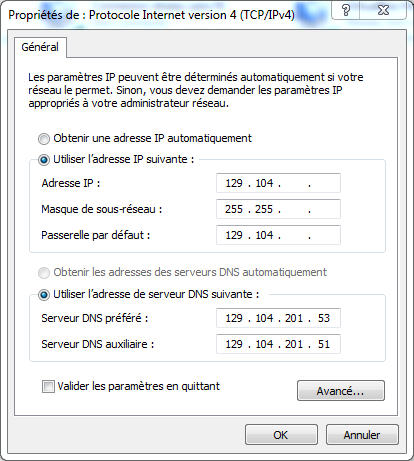
\includegraphics[width=0.48\textwidth]{images/win_config_ip} \label{config:win:IP1}}
%      \hspace{\stretch{1}}
%      \subfloat[Configuration DNS]{ 
%         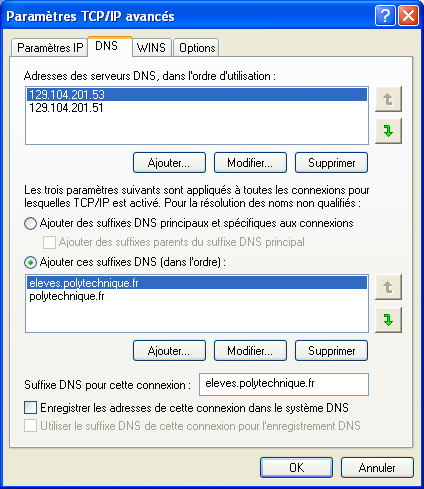
\includegraphics[width=0.48 \textwidth]{images/win_config_dns2} \label{config:win:IP2}}
%             \caption{Configuration réseau}
%    \end{center}
%  \end{figure*}
%
%
%
%%% \newpage
%Coche alors les cases \menu{Utiliser l'adresse IP suivante} et \menu{Utiliser l'adresse de serveur DNS suivante} et remplis les cinq champs d'adresse IP. Tu trouveras toutes les valeurs d'adresse IP nécessaires pour la configuration en page~\pageref{tableau:mon_IP} ; aide-toi de la capture d'écran~\ref{config:win:IP1} pour les placer. Si une partie d'adresse IP est blanche sur cette capture, c'est qu'elle t'est personnelle et que tu dois la calculer !
%Clique ensuite sur le bouton \menu{Avancé}, puis sur l'onglet
%\menu{DNS} en haut.
%Il n'y a plus qu'à  remplir les différents champs comme sur la
%capture d'écran suivante, avec le bouton \menu{Ajouter} et les
%flèches pour réordonner les éléments.
%
%
%%\subsubsection{Le domaine Windows}
%
%%\paragraph{Qu'est ce que c'est ?}
%%Le domaine Windows est un système d'automatisation de la
%%configuration de plusieurs ordinateurs sous Windows situés sur le
%%même réseau. En fait, c'est un outil d'administration, conçu par
%%exemple pour des entreprises où un service informatique doit gérer
%%de nombreuses machines; il permet d'appliquer des modifications de
%%configuration à  toutes les machines du domaine directement depuis un
%%serveur. Le BR possède un serveur dédié au domaine Windows,
%%\server{enez}.
%
%%Le domaine met à  jour automatiquement Windows et l'antivirus à  partir d'\server{enez} (très rapide car tu n'as pas besoin de récupérer des fichiers
%%en dehors de l'école!). Il configure le \emph{firewall} (pare-feu: système de protection contre les éventuelles attaques par le réseau) Windows, mais
%%il est toujours possible de le désactiver si tu préfères un autre \emph{firewall}. En bref, il permet de simplifier à  l'extrême %la mise à  jour
%%continuelle de l'ordinateur.%
%
%
%%\paragraph{Alors, domaine ou pas domaine ?} Soit tu choisis de te
%%mettre sur le domaine Windows, et tu vas alors au paragraphe
%%\guillemotleft~Inscription sur le domaine Windows~\guillemotright.%
%
%%% \newpage
%%\textbf{Avantages :}
%%\begin{itemize}
%%\item Windows est mis à  jour automatiquement ; tu as toujours les
%%dernières corrections de sécurité et un pare-feu correctement
%%configuré. Donc tu es mieux protégé contre les intrusions.
%%\item Surtout, tu n'as plus à  t'en occuper, presque tout est automatique.
%%\end{itemize}%
%
%%\textbf{Inconvénients :}
%%\begin{itemize}
%%  \item Tu délègues une partie des droits d'administration de ta machine au BR
%%        (tout ce qui concerne la sécurité du réseau en particulier).
%%        Cependant, si tu ne sais pas le faire, c'est plutôt un avantage
%%        de laisser le BR s'en occuper à  ta place.
%%  \item Cela ne marche qu'avec Windows 2000, Windows XP Pro ou Windows Vista Business.
%%        On te rappelle que tu peux facilement, gratuitement et légalement passer à 
%%        Windows XP Pro ou bien à  Windows Vista Business (section sur les licences
%%        MSDNAA en page \pageref{msdnaa}).
%%\end{itemize}
%
%%Bien s\^{u}r, tu peux sortir du domaine à  tout instant, et effectuer manuellement les réglages nécessaires à  la sécurité de ton ordinateur.
%
%%Soit tu choisis de configurer toi-même ton ordinateur, et tu peux passer
%%directement à  la section \guillemotleft Installation de l'antivirus
%%\guillemotright. Tu trouveras les informations nécessaires à  la configuration
%%manuelle du pare-feu et du proxy pour \app{Windows Update} en annexe à  la
%%fin de cette section, en page \pageref{horsdomaine}.
%
%%\textbf{Avantage :} Tu es le seul à  t'occuper de la gestion de ton ordinateur.
%
%%\textbf{Inconvénient :} Tu es le seul à  t'occuper de la gestion de ton ordinateur. ;-)
%%S'il devient un foyer pour virus, sache que nous avons les moyens de l'isoler
%%pour éviter toute propagation.
%
%%\begin{center}
%%  \fbox{
%%    \begin{minipage}{.7\textwidth}
%%      \begin{center}
%%Le BR te conseille \emph{très fortement} de te mettre sur le domaine
%%et de choisir l'installation simplifiée !
%%      \end{center}
%%    \end{minipage}
%%  }
%%\end{center}
%
%
%%\paragraph{Inscription sur le domaine Windows}
%
%%On te rappelle que tu ne peux t'inscrire sur le domaine que si tu utilise
%%Windows 2000, Windows XP Pro ou Windows Vista. Si tu possède Windows XP
%%Familial, Windows Vista Home ou encore une version antérieure de Windows,
%%tu dois effectuer toi-même tes réglages de pare-feu et de proxy
%%\app{Windows Update}. Réfère-toi pour cela à  l'annexe ad hoc à  la fin de
%%cette section, en page \pageref{horsdomaine}.
%
%%La procédure d'inscription est la suivante :
%%\begin{itemize}
%
%%\item \textbf{Sous Windows XP :} Clique sur le \menu{Menu Démarrer} puis fais un clic-droit sur
%%\menu{Poste de travail} et choisis \menu{Propriétés}. Ensuite, sélectionne l'onglet \menu{Nom de l'ordinateur} et clique le bouton \menu{Modifier}.
%
%%\item \textbf{Sous Windows Vista :} Clique sur \menu{Menu Démarrer}, puis fais un clic-droit sur \menu{Ordinateur}, \menu{Propriétés}. Là  sélectionne \menu{Paramètres système avancés}, onglet \menu{Nom de l'ordinateur}, puis clique sur le bouton \menu{Modifier}.
%
%%\end{itemize}
%
%%Dans la case \menu{Nom de l'ordinateur}, rentre ton pseudo, puis coche la case \menu{domaine} et
%%rentre \urllink{windows.eleves.polytechnique.fr}. Note bien que l'inscription au domaine te sera
%%refusée par le serveur si quelqu'un d'autre utilise déjà  le même nom d'ordinateur que toi. Par
%%conséquent, essaie d'opter pour un pseudo qui t'identifie de façon claire et unique, par exemple
%%\cmd{NOM\_PRENOM} \footnote{Les Jean Dupont et les Julien Thomas sont priés de trouver autre chose
%%;-)}.
%
%%\imagepos{images/win_config_domaine}{0.5}{S'inscrire sur le domaine windows}{!ht}
%
%%\begin{center}
%%\begin{tabular}{ll}
%% \parbox{.45\textwidth}{
%%  et si tu es rouje 2006 :
%%  \begin{description}
%%    \item[Nom] rouje06
%%    \item[Mot de passe] rouje.2006
%%  \end{description}
% % }
%% & \parbox{.45\textwidth}{
%%  Si tu es jône 2007, tu rentres :
%%  \begin{description}
%%    \item[Nom] jone07
%%    \item[Mot de passe] jone.2007
%%  \end{description}
%%  }
%%\\
%%\end{tabular}
%%\end{center}
%
%%\emph{Attention, ces identifiants servent juste à  t'inscrire sur le
%%domaine. Pour utiliser ton ordinateur, tu devras rentrer au
%%démarrage les mêmes nom d'utilisateur et mot de passe que tu avais
%%avant d'être sur le domaine !}
%%
%%
%%
%%%\paragraph{Installation personnalisée} --- configuration manuelle
%
%%\subparagraph{Configuration antivirus} Le BR, concerné par la
%%sécurité du réseau, te propose un antivirus pour lequel tu n'auras
%%pas à  payer la license pour obtenir les mises à  jour. Bien sà�¿½r,
%%libre à  toi d'utiliser ton anti-virus personnel ; cependant il sera
%%à  ta charge de le mettre à  jour très réguliérement. Pour cela
%%utilise comme proxy : \urllink{http://kuzh} sur le port 8080.
%
%%\emph{Installation de l'anti-virus du BR}\ : Commence par
%%désinstaller tous les antivirus ou firewalls que tu pourrais avoir
%%comme expliqué dans le paragraphe \guillemotleft~Installation simplifiée
%%--- configuration automatique~\guillemotright .
%
%%Puis ouvre ton explorateur Windows et tape :
%%\urllink{$\backslash\backslash$enez$\backslash$antivirus}
%%et double-clique sur le fichier \file{Symantec.exe}.
%
%%Ce package contient le paramétrage de la mise à  jour automatique de
%%Windows sur le serveur de l'école. Attends la fin de l'installation
%%et c'est fini ! Maintenant, tu n'as plus à  toucher à  l'antivirus,
%%normalement il sera mis à  jour automatiquement.
%
%%\subparagraph{Configuration firewall}
%
%%Si tu as Windows XP avec le SP2 installé, tu as un firewall
%%automatiquement activé et facile d'utilisation. En effet, à  chaque
%%fois qu'un programme tentera d'aller pour la première fois sur
%%Internet, il te demandera si tu veux le laisser faire ou non, comme
%%dans la capture~\ref{config:win:firewall}.
%
%%\imageref{images/win_firewall}{0.8}{Un programmme --- ici GuildFTP
%%--- demande à  accéder au réseau}{!ht}{config:win:firewall}
%
%%Le firewall commercial \app{ZoneAlarm}, indépendant de Windows,
%%fonctionne sur le même principe. Tu peux le trouver sur \xshare.
%
%%Si tu préfères utiliser le firewall intégré à  Windows XP (sans le
%%SP2) ou à  Windows Server 2003, il te faudra le configurer en détail.
%%Va dans le \menu{Menu Démarrer}, \menu{Paramètres} et clique sur
%%\menu{Connexions Réseau}. Choisis la connexion qui est utilisée par
%%ton ordinateur (souvent il n'y en a qu'une, ou alors une seule est
%%activée) et double-clique dessus. Clique sur \menu{Propriétés} en
%%bas à  gauche, puis sur l'onglet \menu{Avancé} et rentre dans le menu
%%de \menu{Paramètres} du \menu{Pare-feu Windows}. Il te faudra alors
%%ajouter manuellement tous les ports que tu veux ouvrir sur
%%l'extérieur. Pour cela, clique sur \menu{Ajouter}, et remplis la
%%boà�¿½te de dialogue en t'aidant de la capture
%%d'écran~\ref{config:win:ouvrir_port}; mets le numéro du port que tu
%%veux ouvrir, par exemple 5050, 5053 et 5055 en TCP pour \app{qRezix}
%%et 21 en TCP pour ton FTP.
%
%%\imageref{images/win_config_firewall}{0.7}{Ouvrir un port dans le firewall %Windows}{!ht}{config:win:ouvrir_port}
%
%%Comme tu peux le constater, il est beaucoup plus pratique d'aller
%%sur le domaine et de laisser le SP2 faire le gros du boulot à  ta
%%place :-).
%
%
%
%\subsubsection{Configuration \emph{web} (serveur mandataire)}
%
%\imageref{images/win_config_proxy}{0.5}{Configuration du serveur mandataire (\emph{proxy})}{!ht}{config:win:proxy}
%
%Même si tu n'utilises pas \app{Internet Explorer} comme client \emph{web}, Windows et d'autres programmes
%utilisent ses paramètres, notamment \app{Windows Update}. Par conséquent lance \app{Internet Explorer} et va
%dans le menu \menu{Outils}, \menu{Options Internet}, puis sur l'onglet \menu{Connexions} de la
%nouvelle fenêtre et enfin sur \menu{Paramètres réseau} dans le bas de la fenêtre. Tu dois être arrivé sur une fenêtre semblable à celle de la capture d'écran~\ref{config:win:proxy}. Là, coche
%uniquement la case \menu{Utiliser un script de configuration automatique}, puis remplis le champ
%\menu{Adresse} avec \urllink{http://config/proxy.pac}.
%
%Une fois que tu as fait ça, tu n'as plus forcément besoin d'\app{Internet Explorer}, tu peux donc utiliser un autre navigateur, comme \app{Mozilla
%Firefox}, disponible sur \urllink{http://www.mozilla-europe.org/fr/products/}.
%
%Même si tu ne configures pas Windows Update avec le paragraphe ci-dessous, n'oublie pas de régler ton navigateur \emph{web} et ton client \emph{mail} si tu en as un : reporte-toi page \pageref{browser}.
%
%\subsubsection{Windows Update}
%
%\label{horsdomaine} %\emph{Cette sous-section ne concerne pas les gens qui ont choisi de s'inscrire sur le domaine.}
%
%%\paragraph{Pare-feu} Si tu as Windows XP avec le SP2 installé, ou \emph{a fortiori}
%%Windows Vista, tu as un \emph{firewall} automatiquement activé et facile d'utilisation. En effet, à  chaque fois qu'un programme tentera d'aller pour
%%la première fois sur Internet, il te demandera si tu veux le laisser faire ou non. Si tu préfères une protection indépendante de Windows, le
%%\emph{firewall} commercial \app{Zone\-Alarm} fonctionne sur le même principe. Tu peux le trouver sur \xshare.
%
%%Si tu préfères utiliser le \emph{firewall} intégré à  Windows XP (sans le SP2), il te faudra le configurer en détail. Va dans le \menu{Menu Démarrer},
%%\menu{Paramètres} et clique sur \menu{Connexions Réseau}. Choisis la connexion qui est utilisée par ton ordinateur (souvent il n'y en a qu'une, ou
%%alors une seule est activée) et double-clique dessus. Clique sur \menu{Propriétés} en bas à  gauche, puis sur l'onglet \menu{Avancé} et rentre dans le
%%menu de \menu{Paramètres} du \menu{Pare-feu Windows}. Il te faudra alors ajouter manuellement tous les ports que tu veux ouvrir sur l'extérieur. Pour
%%cela, clique sur \menu{Ajouter}, et remplis la boîte de dialogue% en t'aidant de la capture d'écran~\ref{config:win:ouvrir_port} ci après
%%; mets le numéro du port que tu veux ouvrir, par exemple 5050, 5053 et 5055 en TCP pour \app{qRezix} et 21 en TCP pour ton FTP.
%
%Il reste une dernière configuration de
%serveur mandatataire indispensable pour que puissent se faire les mises à  jour automatiques
%de Windows. Il t'est fortement recommandé de le faire.
%
%\begin{description}
%
%\item[Sous Windows 7 \& Windows 8] Si tu as correctement configuré ton serveur \emph{web} mandataire, les mises à jours se font automatiquement.
%
%\item[Sous Windows XP] Fais \menu{Démarrer}, \menu{Exécuter}, puis
%tape \cmd{cmd} dans la fenêtre qui s'affiche. Une ligne de commande apparaît,
%il te suffit alors de taper : \cmd{proxycfg -p http://kuzh:8080} pour régler
%le serveur mandataire. Pour revenir à  un accès direct il faut taper \cmd{proxycfg -d}.
%
%\item[Sous Windows Vista]
%Dans le menu \menu{Démarrer}, tape \guillemotleft~Invite de commandes~\guillemotright{} dans le champ \menu{Rechercher}, puis clique droit sur le lien
%et choisis \menu{Exécuter en tant qu'administrateur}. Tape ensuite les commandes suivantes :
%\cmdline{
%C:\textbackslash{}Windows\textbackslash{}system32$>$netsh\\
%netsh>winhttp\\
%netsh winhttp>set proxy proxy-server="http://kuzh:8080"\\
%netsh winhttp>exit\\
%C:\textbackslash{}Windows\textbackslash{}system32>exit }
%
%Pour revenir à l'accès direct, il suffit de taper :
%\cmdline{
%  netsh winhttp reset proxy
%}
%
%Pour la suite de ta configuration, rendez-vous page \pageref{browser} pour faire marcher ton navigateur web préféré !
%
%\end{description}

%\clearpage